\documentclass[11pt,a4paper]{article}

\usepackage[margin=22mm]{geometry}
\usepackage[T1]{fontenc}
\usepackage[utf8]{inputenc}
\usepackage{lmodern}
\usepackage{microtype}
\usepackage{amsmath}
\usepackage{booktabs}
\usepackage{array}
\usepackage{tabularx}
\usepackage{graphicx}
\usepackage{float}
\usepackage{caption}
\usepackage{subcaption}
\usepackage{xcolor}
\usepackage{hyperref}
\usepackage{fancyhdr}
\emergencystretch=3em

\hypersetup{
  colorlinks=true,
  linkcolor=black,
  urlcolor=blue!50!black,
  citecolor=black,
  pdftitle={Blade Concept Matrix},
  pdfauthor={implicit-geometry-kernel}
}

\graphicspath{%
  {../../../examples/blade/09_blade_concepts/figures/}%
  {../../../examples/demos/figures/structural_family_grids/}%
}

\newcommand{\tok}[1]{\texttt{#1}}
\newcommand{\code}[1]{\texttt{#1}}
\newcolumntype{L}[1]{>{\raggedright\arraybackslash}p{#1}}

\captionsetup{font=small,labelfont=bf,skip=6pt}

\pagestyle{fancy}
\fancyhf{}
\lhead{\small Blade Concept Matrix}
\rhead{\small implicit-geometry-kernel}
\cfoot{\thepage}

\title{Blade Concept Matrix}
\author{implicit-geometry-kernel\\
  \normalsize Companion to \texttt{docs/blade/concepts/taxonomy.md}}
\date{}

\begin{document}
\maketitle
\thispagestyle{fancy}

\begin{abstract}
\noindent
A catalogue key names a blade concept. The Markdown page is canonical;
figures below are example~09 cutaways unless noted.
\end{abstract}

\section{Concept Catalogue}

\begin{verbatim}
[W][X]-[Y]-[Z]-[R]     e.g.  2D-F-LC-0R    2D-F-LE-10R    2D-F-PA-10R
 |  |   |   |   +-- rib count (required NR): n = 0..10 (figures: 0R · 4R · 10R)
 |  |   |   +------ web anchoring (required): LC | LE | PA
 |  |   +---------- web orientation: F flapwise | CN chord-normal
 |  +-------------- spar-cap family: A B C D
 +----------------- web count: 0..5
\end{verbatim}

Zero-web cores omit $[Y]$: \tok{0A-LC-0R}, \tok{0A-LE-10R}. Bare \tok{2D-F} and
omitted \tok{0R} are invalid.
\code{BladeConcept.from\_key("2D-F-LC-0R")} /
\code{resolve\_system\_type(...)} yields a frozen \code{SystemLayoutSpec}.

\begin{table}[H]
\centering
\caption{Concept letters.}
\label{tab:parts}
\begin{tabularx}{\textwidth}{@{}llX@{}}
\toprule
Part & Meaning & Examples \\
\midrule
\textbf{W} & Shear-web count & \tok{0} \tok{1} \tok{2} \ldots \tok{5} \\
\textbf{X} & Spar-cap family & \tok{A} \tok{B} \tok{C} \tok{D} \\
\textbf{Y} & Web orientation & \tok{CN} \tok{F} (omit when $W=0$) \\
\textbf{Z} & Web anchoring & \tok{LC} \tok{LE} \tok{PA} \\
\textbf{R} & Rib count (required \tok{NR})
  & integer $0\ldots 10$; figures \tok{0R} \tok{4R} \tok{10R} \\
\bottomrule
\end{tabularx}
\end{table}

\section{\texorpdfstring{$W$}{W} --- web count}
\label{sec:w}

Fixed $X=\mathrm{D}$, $Y=\mathrm{F}$, $Z=\mathrm{PA}$, $R=10$.
Two-web \tok{2D-F-PA-10R} is under $Z$.

\begin{figure}[H]
\centering
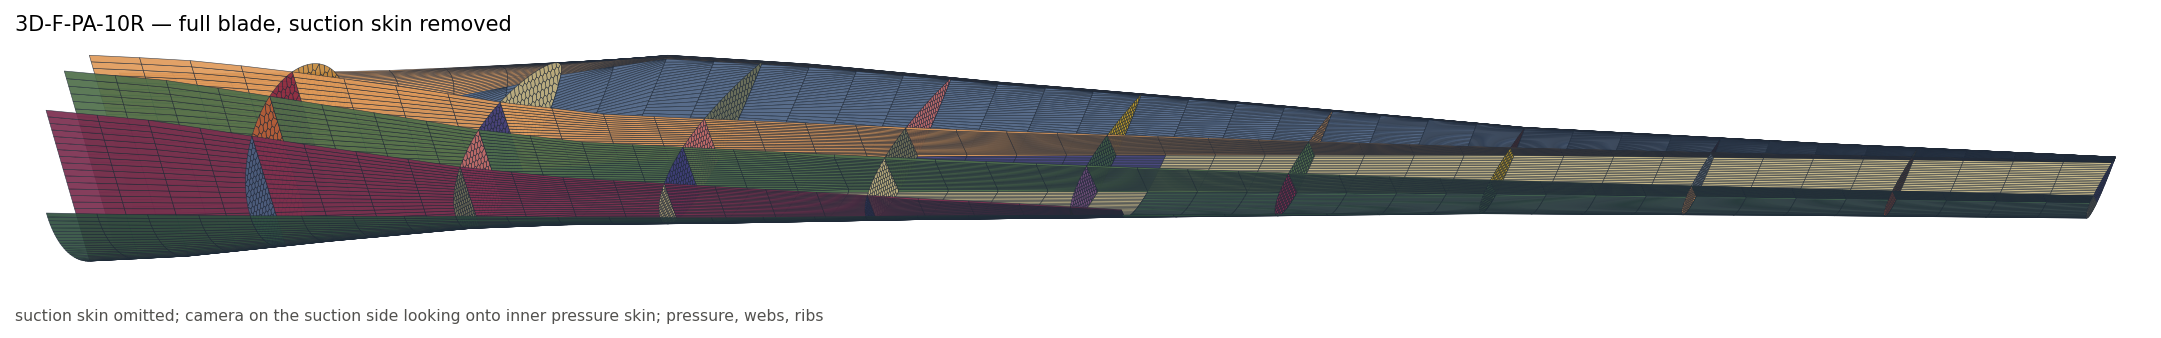
\includegraphics[width=\textwidth]{3D-F-PA-10R/full_blade/cutaway.png}
\caption{\tok{3D-F-PA-10R}: three webs.}
\label{fig:w-3}
\end{figure}

\begin{figure}[H]
\centering
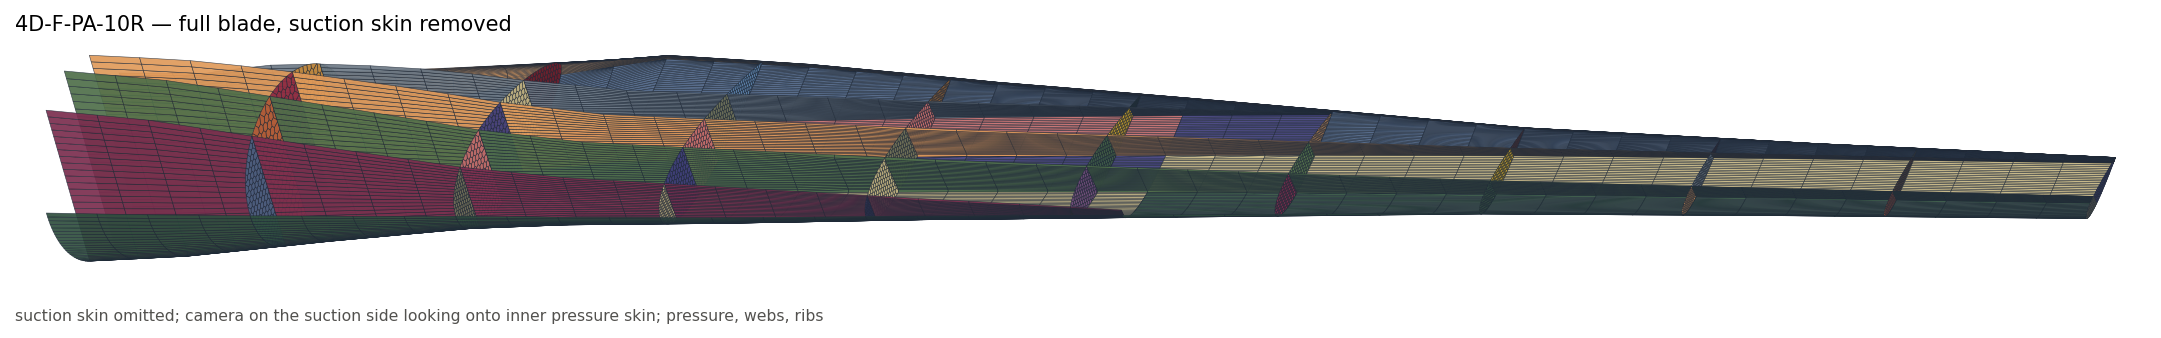
\includegraphics[width=\textwidth]{4D-F-PA-10R/full_blade/cutaway.png}
\caption{\tok{4D-F-PA-10R}: four webs.}
\label{fig:w-4}
\end{figure}

\begin{figure}[H]
\centering
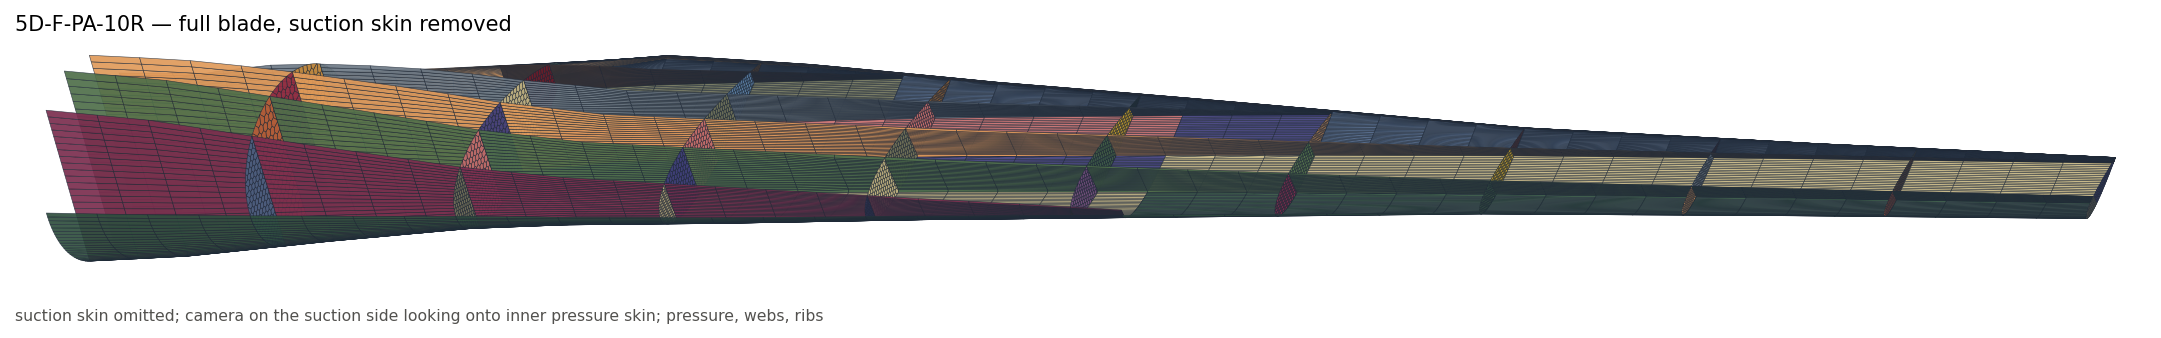
\includegraphics[width=\textwidth]{5D-F-PA-10R/full_blade/cutaway.png}
\caption{\tok{5D-F-PA-10R}: five webs.}
\label{fig:w-5}
\end{figure}

\section{\texorpdfstring{$X$}{X} --- spar-cap families}
\label{sec:x}

\begin{table}[H]
\centering
\caption{Spar-cap families.}
\label{tab:x-families}
\begin{tabular}{@{}c L{0.82\textwidth}@{}}
\toprule
$X$ & Description \\
\midrule
\textbf{A} & No spar caps: skin, webs, cores (and optional inserts) only. \\
\textbf{B} & \textbf{Single} fixed upper/lower cap pair on \textbf{one}
  chordwise band. Anchor: \textbf{pitching} (default $\sim\tfrac13$ chord from
  LE) or \textbf{max\_thickness}. \\
\textbf{C} & \textbf{Multiple} discrete upper/lower cap patches --- one band
  per web --- merged as \code{spar\_cap\_suction\_surface} /
  \code{spar\_cap\_pressure\_surface}. \\
\textbf{D} & \textbf{Continuous box} spar spanning leftmost to rightmost web
  (needs $W\geq 2$; no \tok{1D-*}). \\
\bottomrule
\end{tabular}
\end{table}

\begin{figure}[H]
\centering
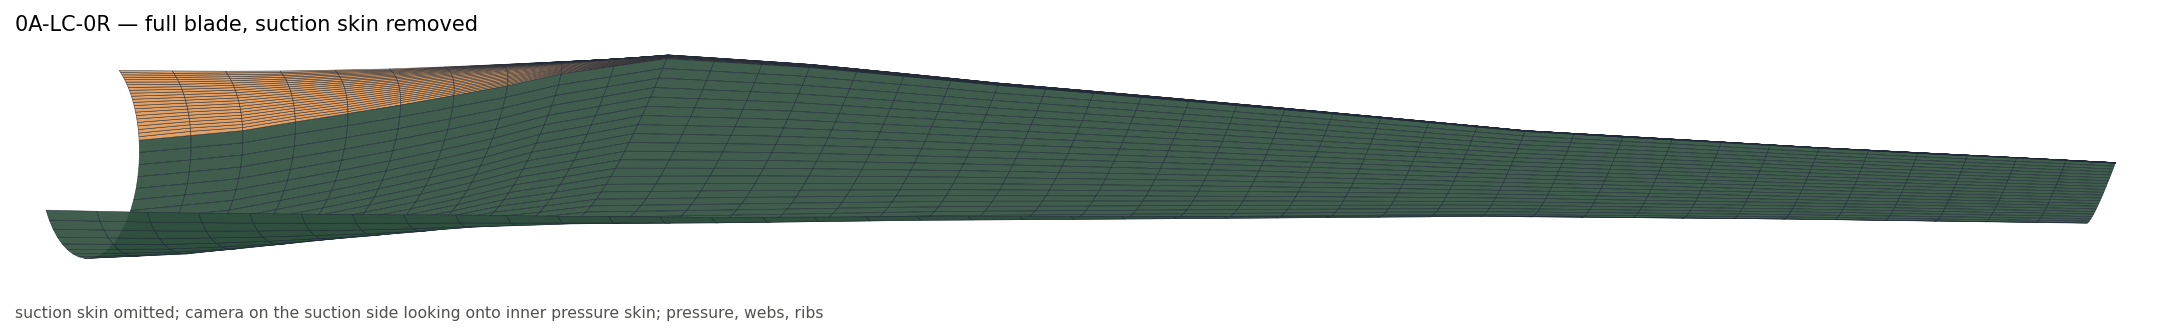
\includegraphics[width=\textwidth]{0A-LC-0R/full_blade/cutaway.png}
\caption{\tok{0A-LC-0R}: family $A$, zero webs.}
\label{fig:x-0a}
\end{figure}

\begin{figure}[H]
\centering
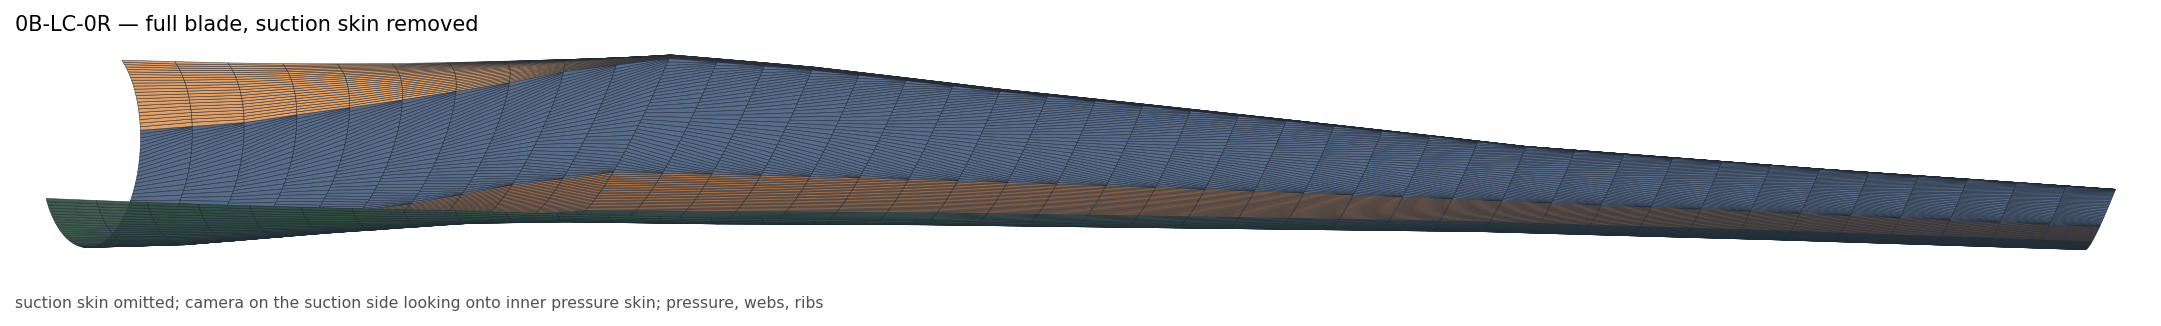
\includegraphics[width=\textwidth]{0B-LC-0R/full_blade/cutaway.png}
\caption{\tok{0B-LC-0R}: family $B$, zero webs, one cap band.}
\label{fig:x-0b}
\end{figure}

\begin{figure}[H]
\centering
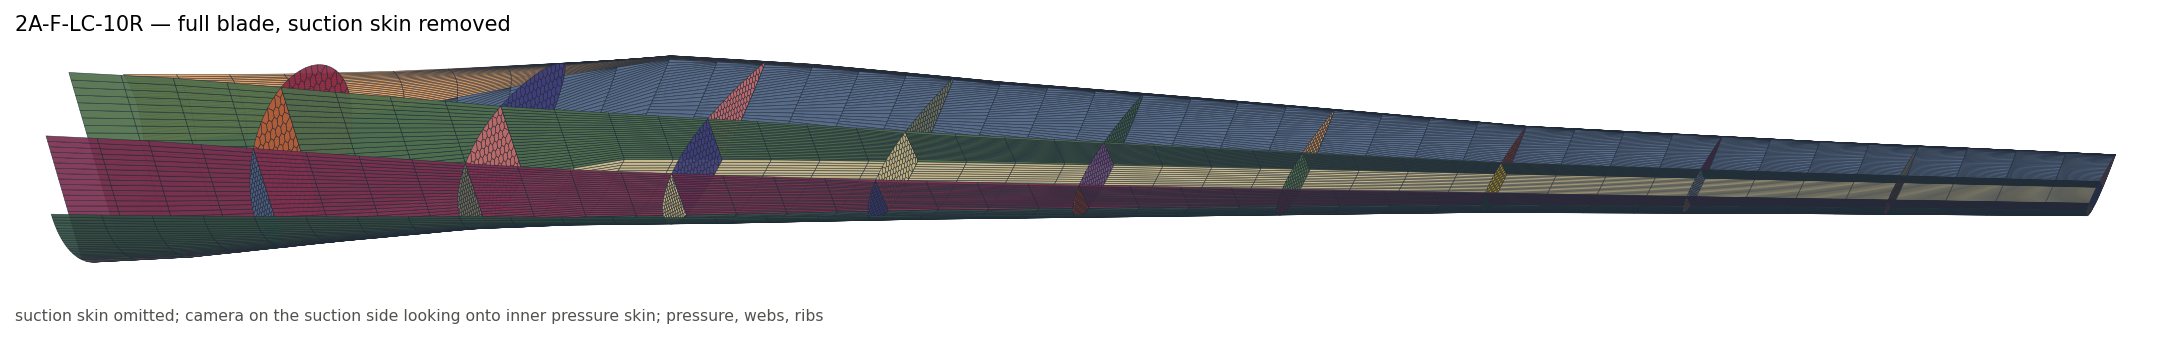
\includegraphics[width=\textwidth]{2A-F-LC-10R/full_blade/cutaway.png}
\caption{\tok{2A-F-LC-10R}: family $A$, two flapwise webs, no caps.}
\label{fig:x-2a}
\end{figure}

\begin{figure}[H]
\centering
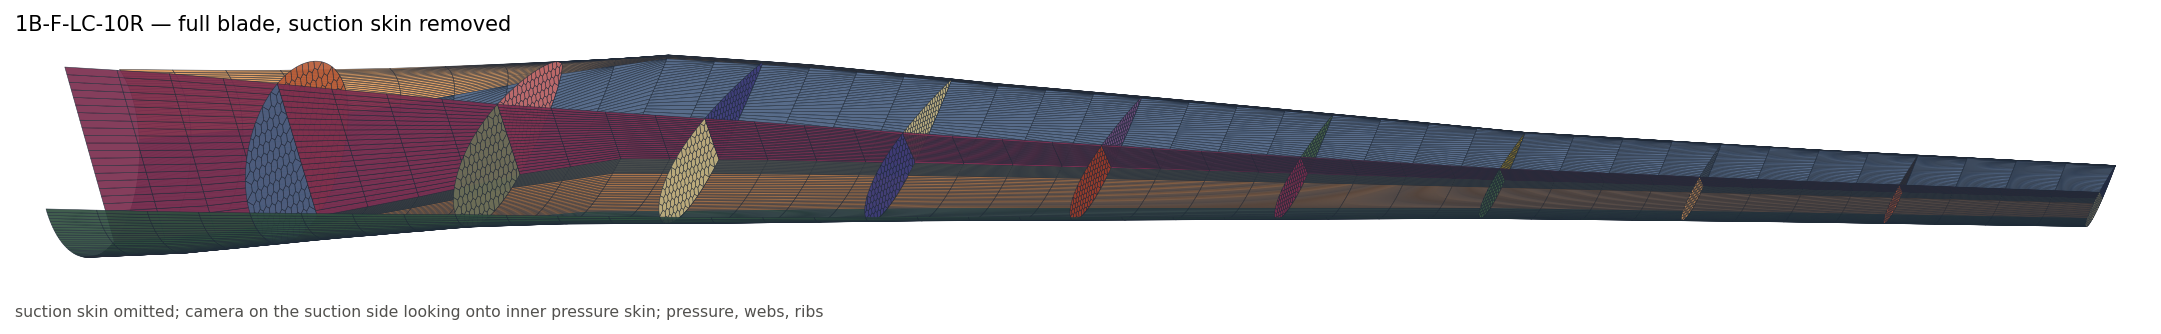
\includegraphics[width=\textwidth]{1B-F-LC-10R/full_blade/cutaway.png}
\caption{\tok{1B-F-LC-10R}: family $B$, one flapwise web, one cap band.}
\label{fig:x-1b}
\end{figure}

\begin{figure}[H]
\centering
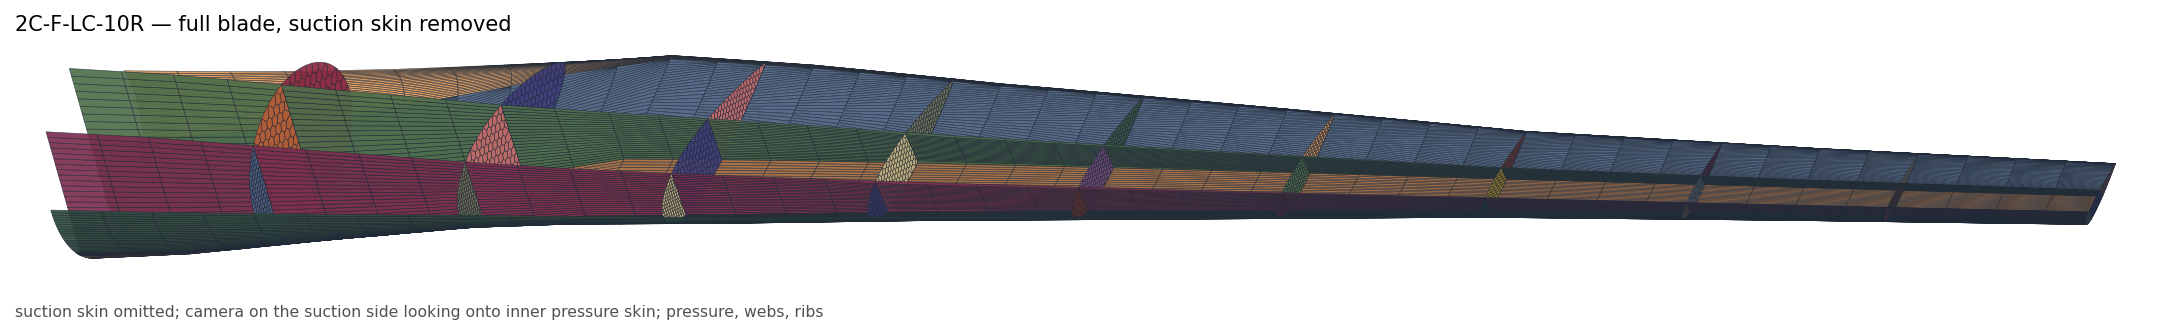
\includegraphics[width=\textwidth]{2C-F-LC-10R/full_blade/cutaway.png}
\caption{\tok{2C-F-LC-10R}: family $C$, per-web cap bands.}
\label{fig:x-2c}
\end{figure}

\begin{figure}[H]
\centering
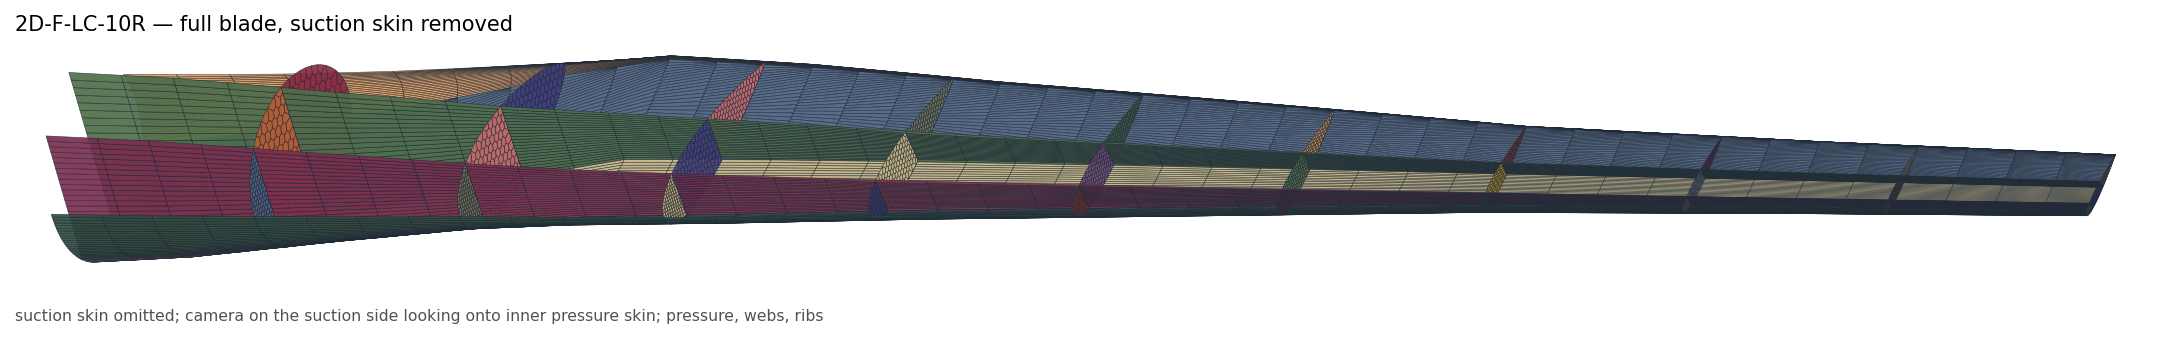
\includegraphics[width=\textwidth]{2D-F-LC-10R/full_blade/cutaway.png}
\caption{\tok{2D-F-LC-10R}: family $D$, continuous box (also $Y=\mathrm{F}$,
  $Z=\mathrm{LC}$, $R=10$).}
\label{fig:x-2d}
\end{figure}

\section{\texorpdfstring{$Y$}{Y} --- web orientation}
\label{sec:y}

\begin{table}[H]
\centering
\caption{Web orientation. Station slices; tilt is not obvious in a full-blade
cutaway.}
\label{tab:y}
\begin{tabularx}{\textwidth}{@{}cX@{}}
\toprule
$Y$ & Meaning \\
\midrule
\textbf{CN} & Chord-normal in the \textbf{untwisted} section. \\
\textbf{F} & Vertical in the \textbf{twisted} blade frame (flapwise). \\
\bottomrule
\end{tabularx}
\end{table}

\begin{figure}[H]
\centering
\begin{subfigure}[t]{0.48\textwidth}
  \centering
  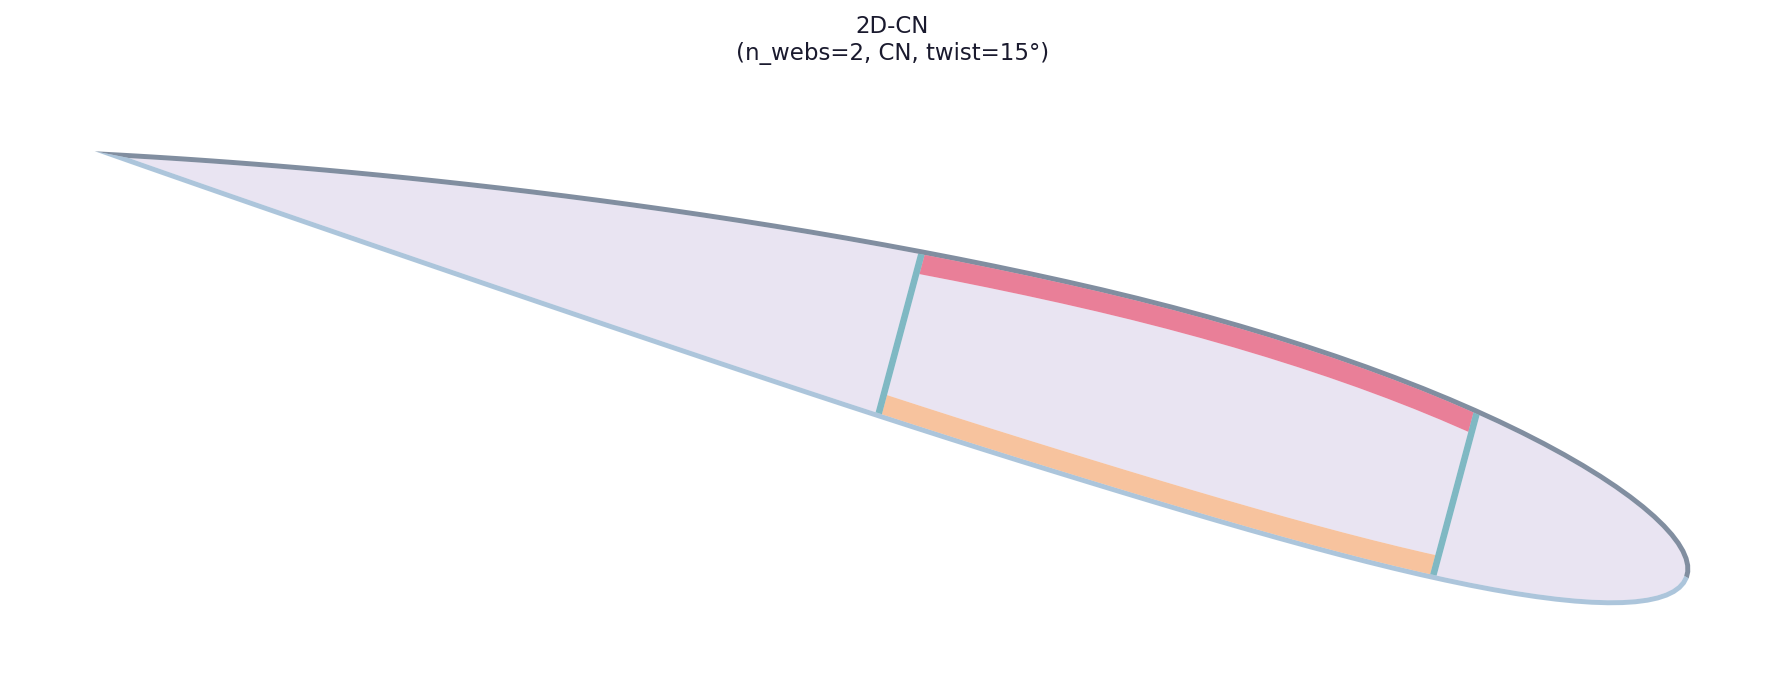
\includegraphics[width=\linewidth]{2D-CN.png}
  \caption{\tok{2D-CN}: chord-normal.}
  \label{fig:y-cn}
\end{subfigure}\hfill
\begin{subfigure}[t]{0.48\textwidth}
  \centering
  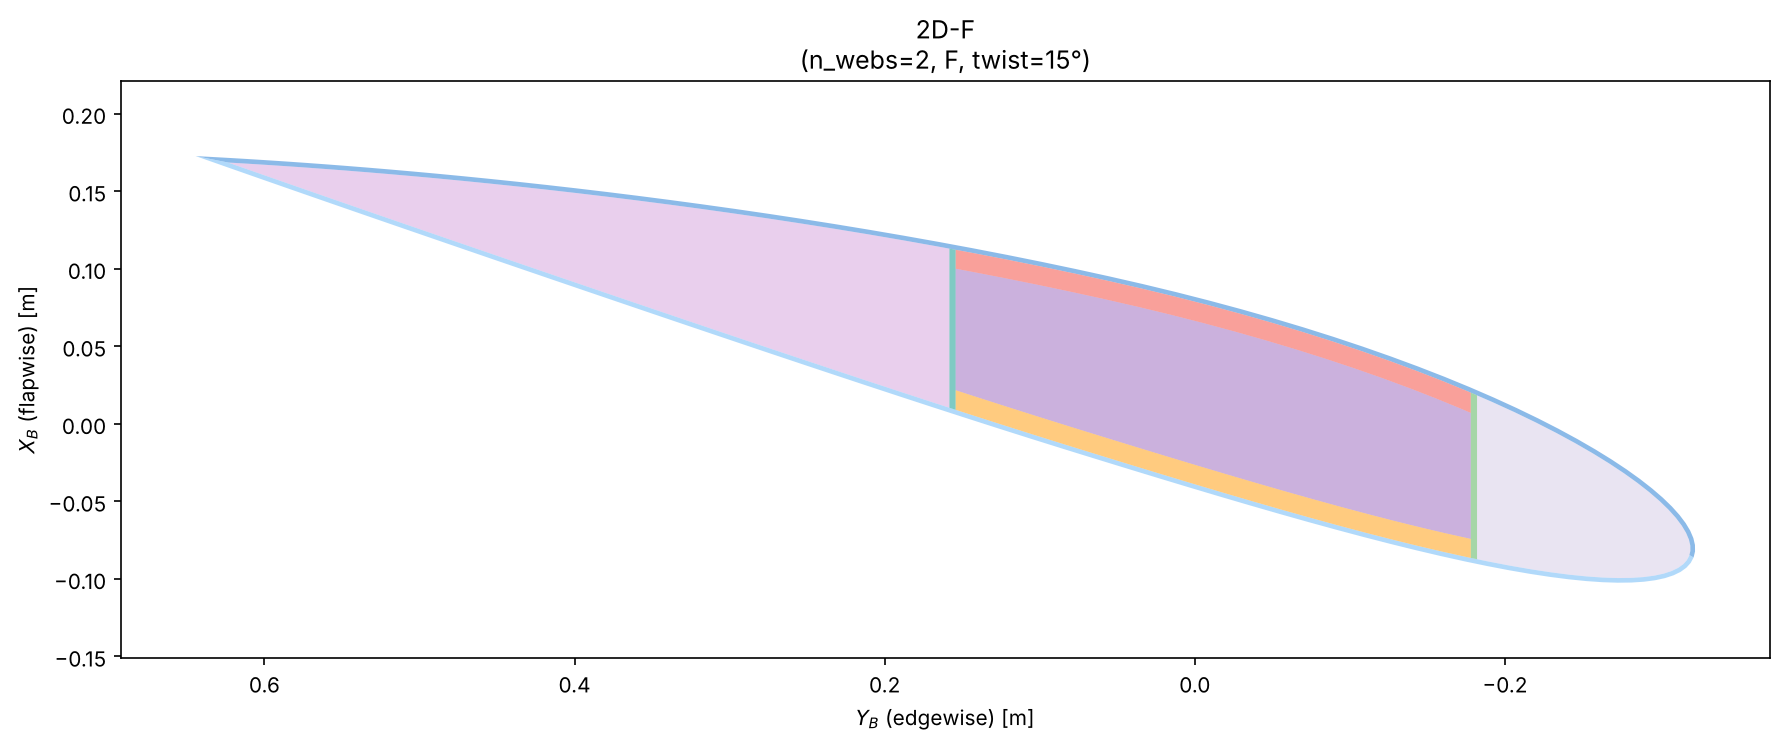
\includegraphics[width=\linewidth]{2D-F.png}
  \caption{\tok{2D-F}: flapwise.}
  \label{fig:y-f}
\end{subfigure}
\caption{Web orientation at the station
(\code{examples/demos/figures/structural\_family\_grids/}).}
\label{fig:y-cn-f}
\end{figure}

\section{\texorpdfstring{$Z$}{Z} --- web anchoring}
\label{sec:z}

\begin{table}[H]
\centering
\caption{Web anchoring.}
\label{tab:z}
\begin{tabularx}{\textwidth}{@{}c L{3.4cm} X@{}}
\toprule
$Z$ & Native unit & Span behaviour \\
\midrule
\textbf{LC} & Chord fraction from LE
  & Stations slide with local chord $c(z)$. \\
\textbf{LE} & Metres from leading edge
  & Offset is frozen from the root chord; the web is omitted when it
    misses the inner skin. \\
\textbf{PA} & Blade-frame offset from the pitch axis
  & Constant $x$; primary slots are uniform interiors of the root
    LE--TE band. Extra slots continue that lattice (first extra at root TE). \\
\bottomrule
\end{tabularx}
\end{table}

\begin{figure}[H]
\centering
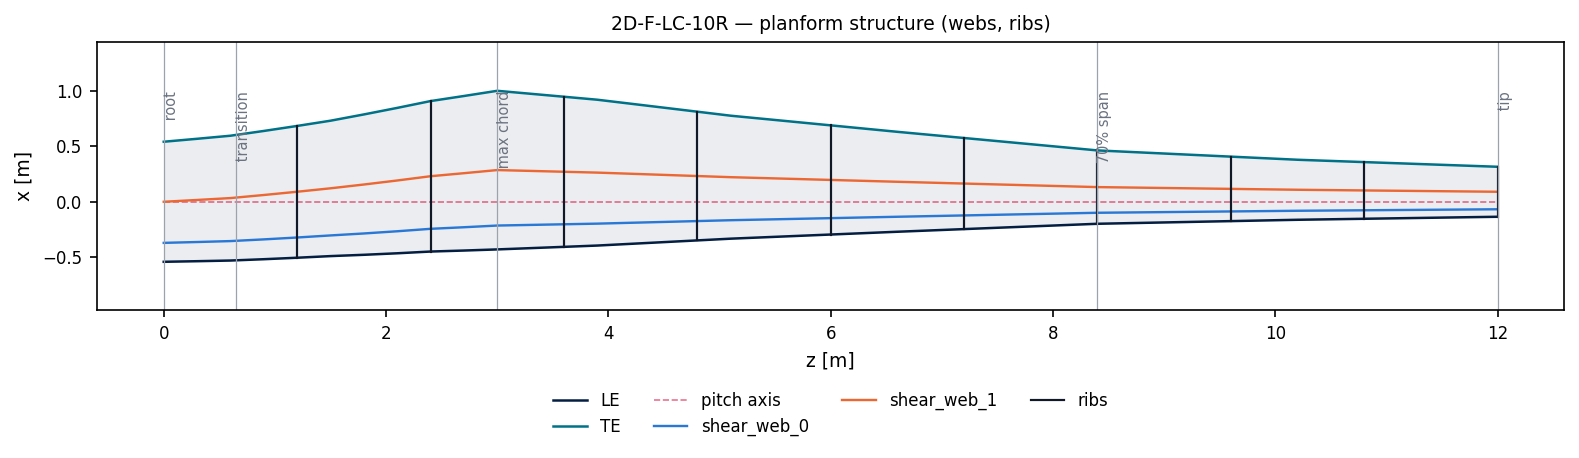
\includegraphics[width=\textwidth]{2D-F-LC-10R/planform/structure.png}
\caption{\tok{2D-F-LC-10R}: loci follow local chord.}
\label{fig:z-2d-lc}
\end{figure}

\begin{figure}[H]
\centering
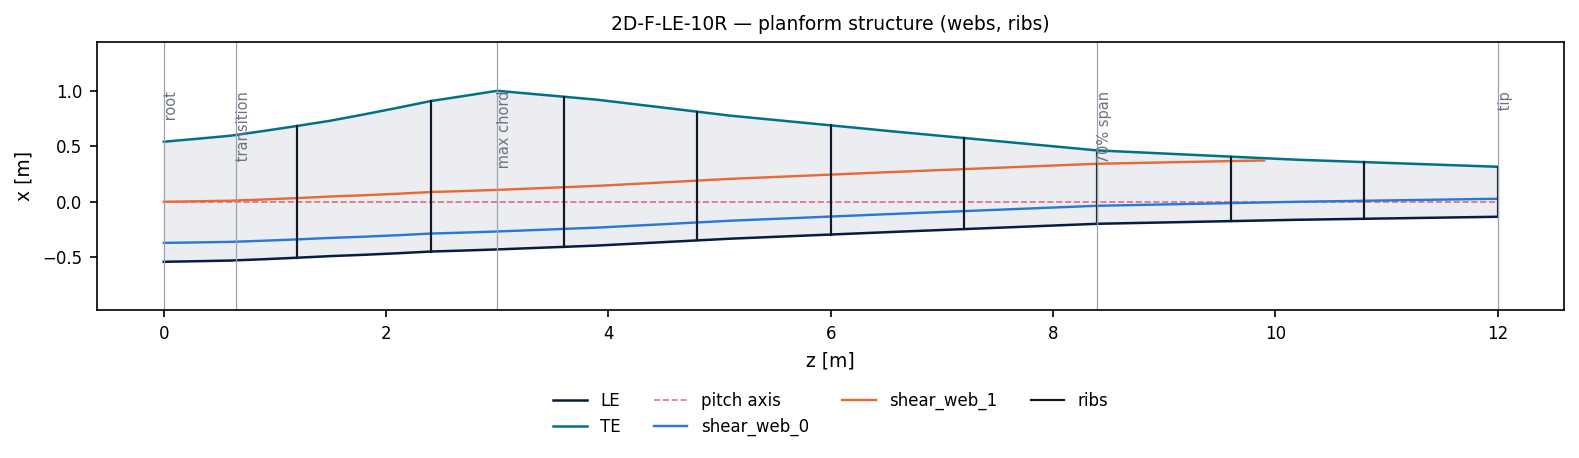
\includegraphics[width=\textwidth]{2D-F-LE-10R/planform/structure.png}
\caption{\tok{2D-F-LE-10R}: leading-edge freeze.}
\label{fig:z-2d-le}
\end{figure}

\begin{figure}[H]
\centering
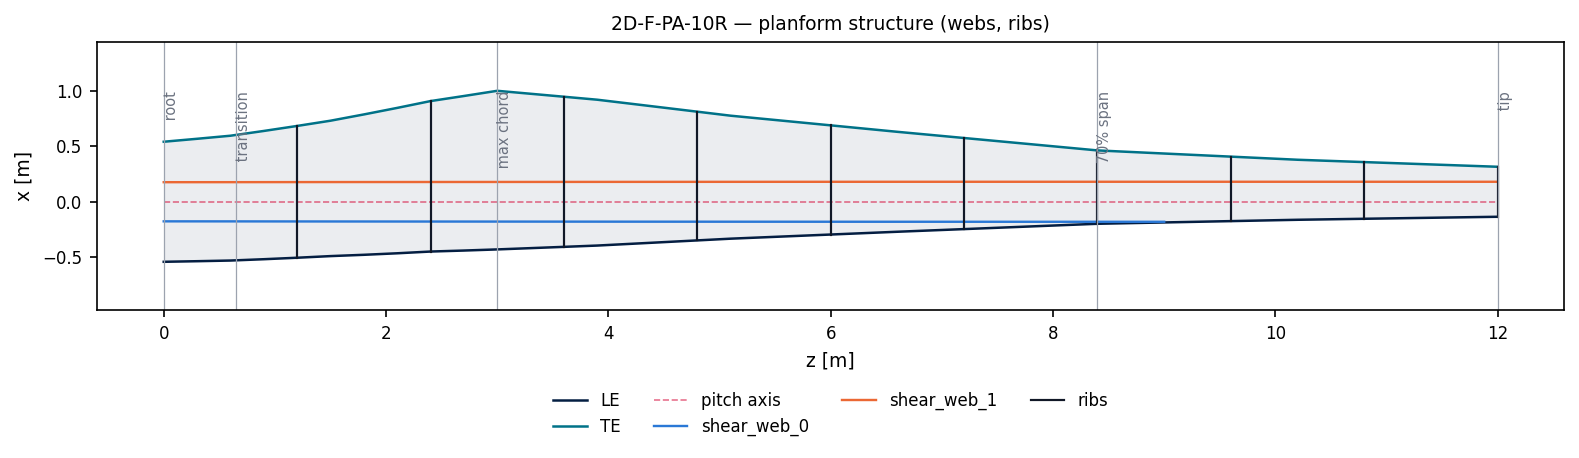
\includegraphics[width=\textwidth]{2D-F-PA-10R/planform/structure.png}
\caption{\tok{2D-F-PA-10R}: pitch-axis freeze.}
\label{fig:z-2d-pa}
\end{figure}

\begin{figure}[H]
\centering
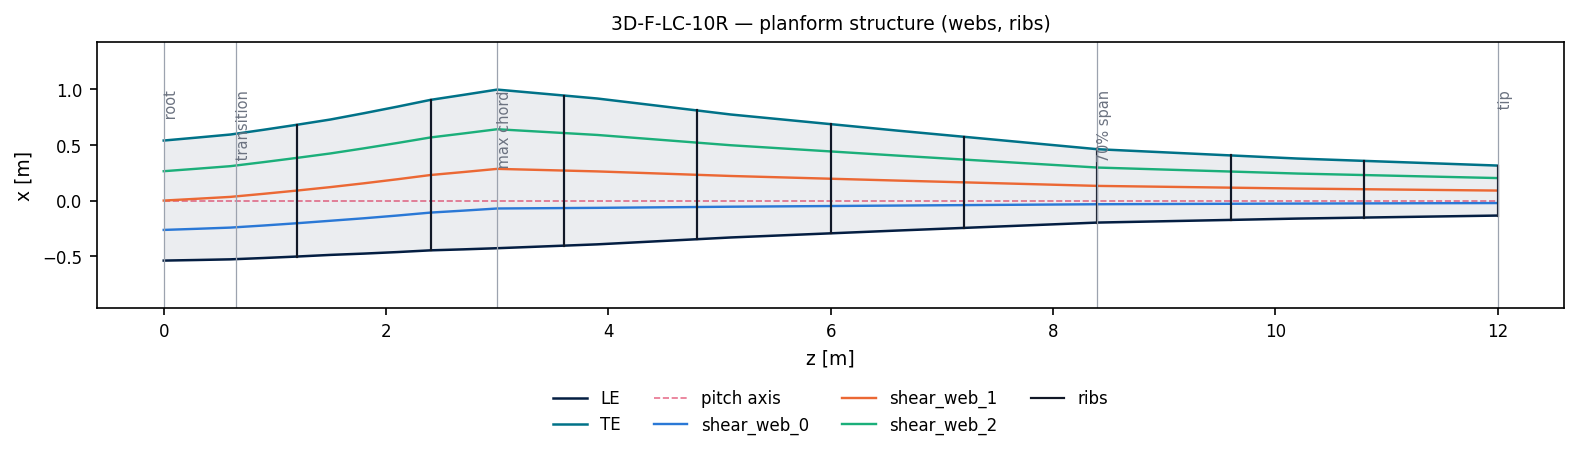
\includegraphics[width=\textwidth]{3D-F-LC-10R/planform/structure.png}
\caption{\tok{3D-F-LC-10R}: three webs, local chord.}
\label{fig:z-3d-lc}
\end{figure}

\begin{figure}[H]
\centering
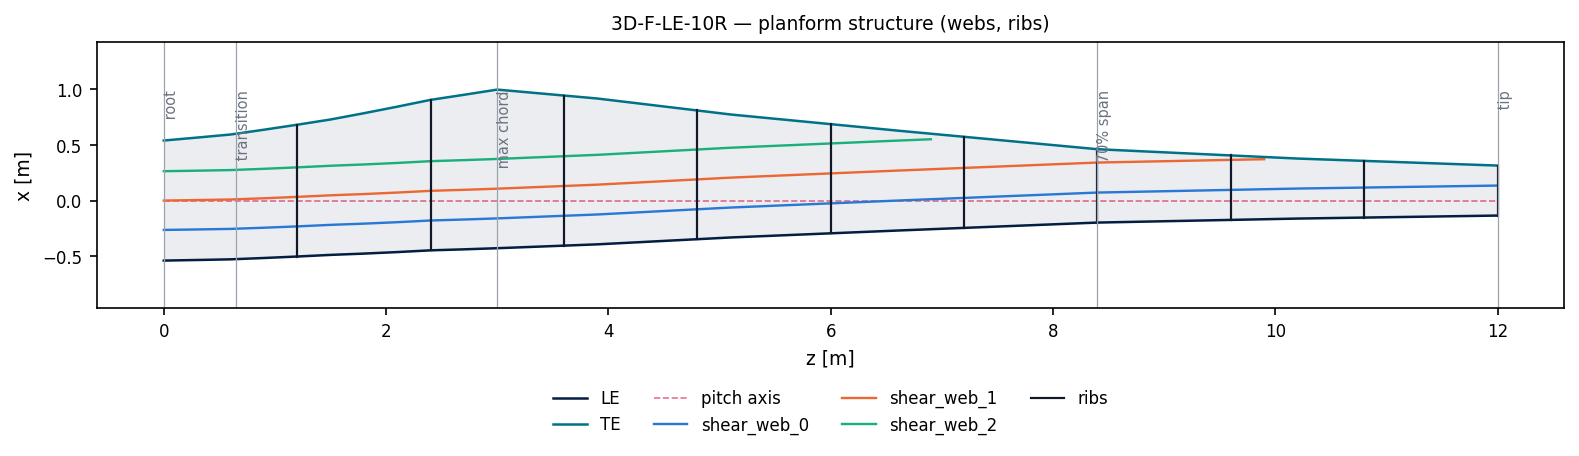
\includegraphics[width=\textwidth]{3D-F-LE-10R/planform/structure.png}
\caption{\tok{3D-F-LE-10R}: three webs, leading-edge freeze.}
\label{fig:z-3d-le}
\end{figure}

\begin{figure}[H]
\centering
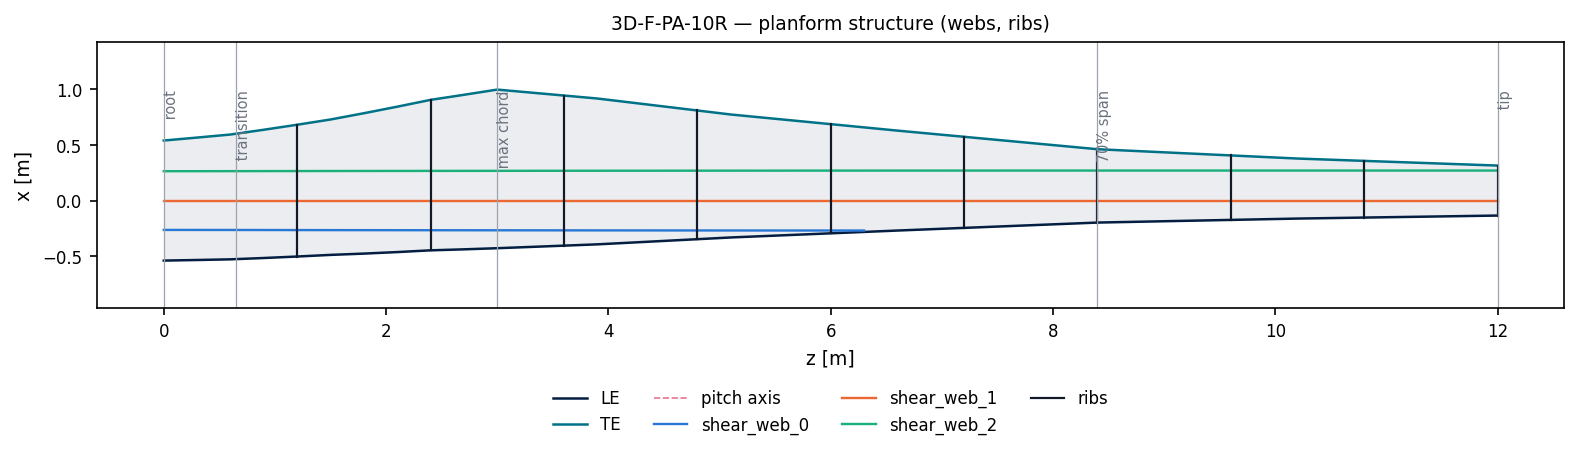
\includegraphics[width=\textwidth]{3D-F-PA-10R/planform/structure.png}
\caption{\tok{3D-F-PA-10R}: three webs, pitch-axis freeze.}
\label{fig:z-3d-pa}
\end{figure}

\begin{figure}[H]
\centering
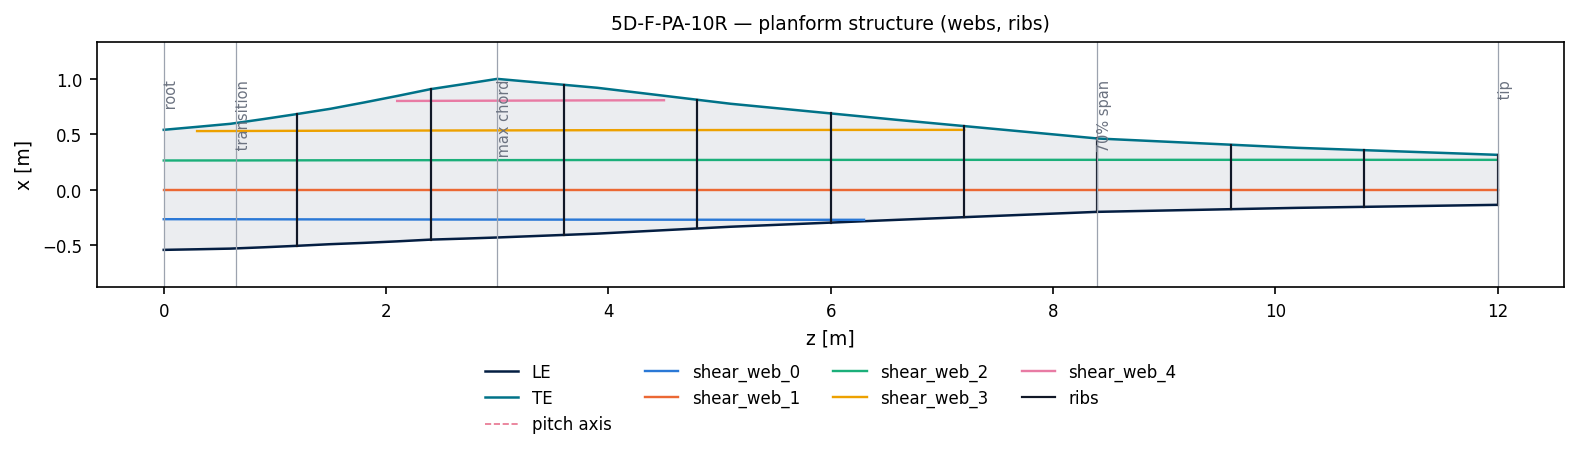
\includegraphics[width=\textwidth]{5D-F-PA-10R/planform/structure.png}
\caption{\tok{5D-F-PA-10R}: five-web pitch-axis lattice.}
\label{fig:z-5d-pa}
\end{figure}

\section{\texorpdfstring{$R$}{R} --- rib count}
\label{sec:r}

\begin{table}[H]
\centering
\caption{Rib count. $n=0\ldots 10$. This lookup shows none and four;
  \tok{10R} is \tok{2D-F-LC-10R} under $X$.
  \code{SYSTEM\_TYPE\_KEYS} enumerates \tok{0R} only.}
\label{tab:r}
\begin{tabularx}{\textwidth}{@{}cX@{}}
\toprule
$R$ & Meaning \\
\midrule
$n$ & Integer transverse-face count $0\ldots 10$.
  Illustrated: \tok{0R} none, \tok{4R} four, \tok{10R} ten. \\
\bottomrule
\end{tabularx}
\end{table}

\begin{figure}[H]
\centering
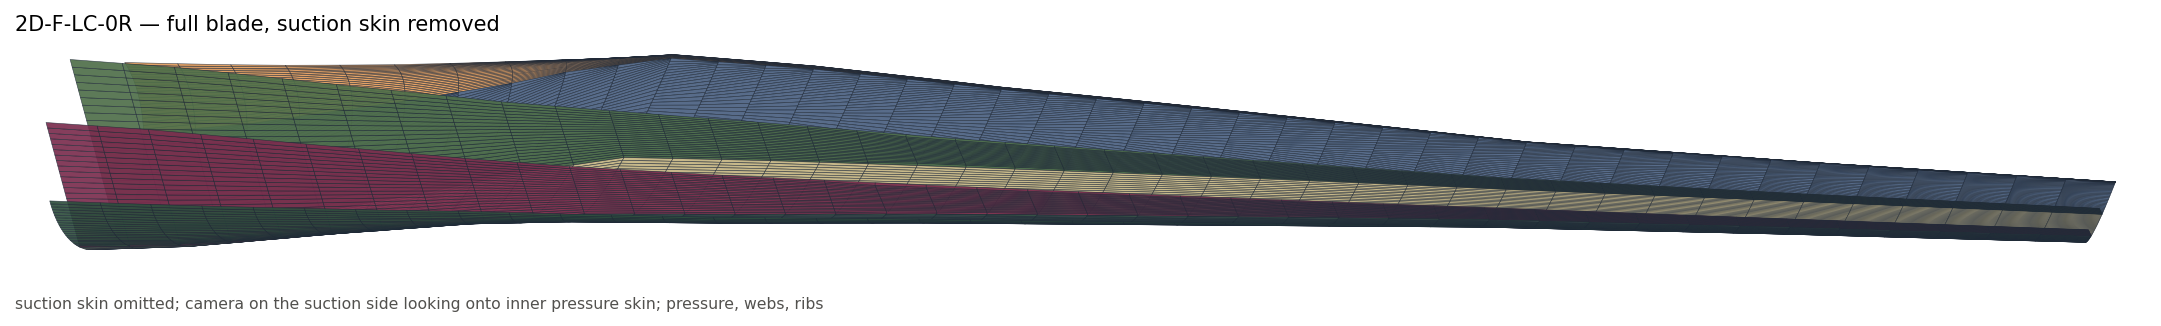
\includegraphics[width=\textwidth]{2D-F-LC-0R/full_blade/cutaway.png}
\caption{\tok{2D-F-LC-0R}: no ribs.}
\label{fig:r-0}
\end{figure}

\begin{figure}[H]
\centering
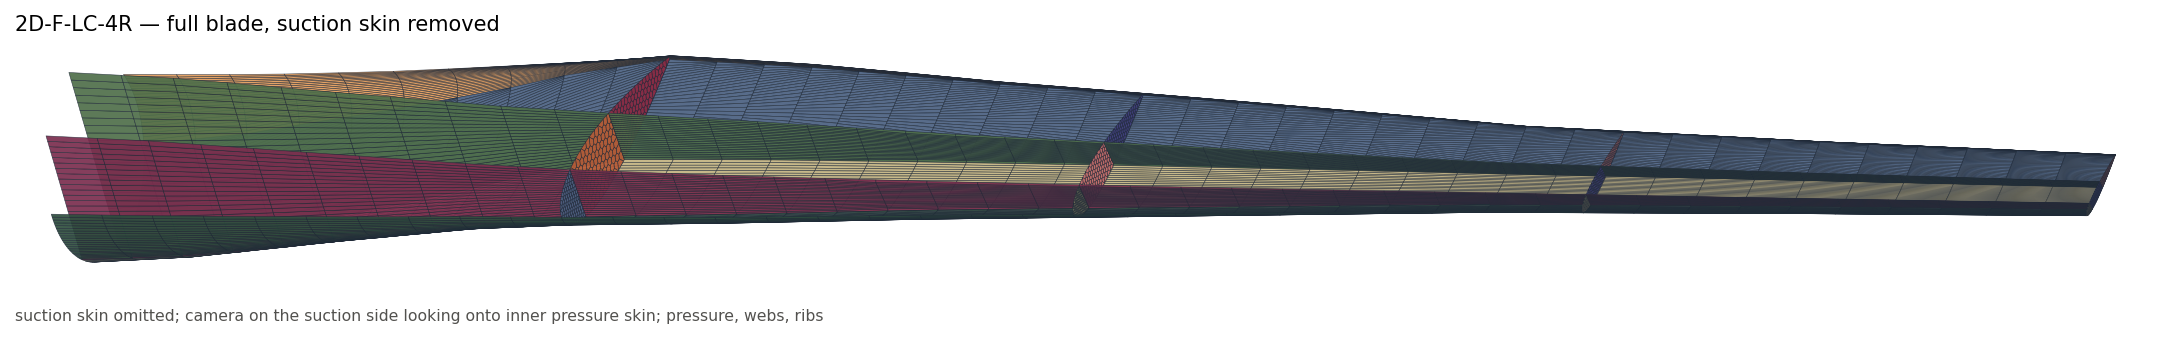
\includegraphics[width=\textwidth]{2D-F-LC-4R/full_blade/cutaway.png}
\caption{\tok{2D-F-LC-4R}: four rib faces.}
\label{fig:r-4}
\end{figure}

\section{Stationwise, spanwise, transverse}
\label{sec:axes}

A concept has three axes. \code{resolve\_system\_type} returns that whole spec.

\begin{table}[H]
\centering
\caption{Blade-concept axes.}
\label{tab:axes}
\begin{tabularx}{\textwidth}{@{}l l X@{}}
\toprule
Axis & Letters & Fixes \\
\midrule
Stationwise & $WXY$ & Web count, cap family, tilt at a cut. \\
Spanwise & $Z$ & Web $x(z)$: \tok{LC} slides, \tok{LE}/\tok{PA} freeze. \\
Transverse & $R$ & Rib-face count $0\ldots 10$. \\
\bottomrule
\end{tabularx}
\end{table}

\begin{table}[H]
\centering
\caption{Stationwise: 40 cores. Empty cells forbidden (no \tok{0C}/\tok{0D},
no \tok{1D}). Attach \tok{-Z-NR} to make a key.}
\label{tab:registry}
\small
\begin{tabular}{@{}c *{8}{c}@{}}
\toprule
$W$ & \tok{A-CN} & \tok{A-F} & \tok{B-CN} & \tok{B-F}
    & \tok{C-CN} & \tok{C-F} & \tok{D-CN} & \tok{D-F} \\
\midrule
0 & \multicolumn{2}{c}{\tok{0A} (no $Y$)}
  & \multicolumn{2}{c}{\tok{0B} (no $Y$)}
  & \multicolumn{2}{c}{---}
  & \multicolumn{2}{c}{---} \\
1 & \tok{1A-CN} & \tok{1A-F} & \tok{1B-CN} & \tok{1B-F}
  & \tok{1C-CN} & \tok{1C-F} & --- & --- \\
2 & \tok{2A-CN} & \tok{2A-F} & \tok{2B-CN} & \tok{2B-F}
  & \tok{2C-CN} & \tok{2C-F} & \tok{2D-CN} & \tok{2D-F} \\
3 & \tok{3A-CN} & \tok{3A-F} & \tok{3B-CN} & \tok{3B-F}
  & \tok{3C-CN} & \tok{3C-F} & \tok{3D-CN} & \tok{3D-F} \\
4 & \tok{4A-CN} & \tok{4A-F} & \tok{4B-CN} & \tok{4B-F}
  & \tok{4C-CN} & \tok{4C-F} & \tok{4D-CN} & \tok{4D-F} \\
5 & \tok{5A-CN} & \tok{5A-F} & \tok{5B-CN} & \tok{5B-F}
  & \tok{5C-CN} & \tok{5C-F} & \tok{5D-CN} & \tok{5D-F} \\
\bottomrule
\end{tabular}
\end{table}

\begin{table}[H]
\centering
\caption{Spanwise: parent concept stays on \code{SectionCut.layout}.
Webs that miss are \textbf{dropped}, not slid; live $W$/$X$ is the station
slice, e.g.\ \tok{4D-F-PA-10R | W=1 X=C dropped=(0,1,2)}.
$Y$, $Z$ and $R$ are not rungs. \tok{0A}/\tok{0B} are authored, not drop targets.}
\label{tab:floors}
\begin{tabularx}{\textwidth}{@{}cX@{}}
\toprule
$X$ & Floor (live webs) \\
\midrule
A & $n\mathrm{A}\to\cdots\to 1\mathrm{A}$ \\
B & $n\mathrm{B}\to\cdots\to 1\mathrm{B}$ \\
C & $n\mathrm{C}\to\cdots\to 1\mathrm{C}$ \\
D & $n\mathrm{D}\to\cdots\to 2\mathrm{D}\to 1\mathrm{C}$ \\
\bottomrule
\end{tabularx}
\end{table}

\noindent
Transverse: $R$ is copied from the parent.
\code{SYSTEM\_TYPE\_KEYS} is the 40 stationwise cores $\times$
$\{\mathrm{LC},\mathrm{LE},\mathrm{PA}\}$ $\times$ \tok{0R} (120 goldens).
\tok{1R}--\tok{10R} resolve.

\end{document}
